\chapter{Introduction}\label{chapintro}

\begin{objectives} \label[objectives]{Introduce-and-motivate-th}

\begin{itemize}
\tightlist
\item
  Introduce and motivate the study of computation for its own sake,
  irrespective of particular implementations.
\item
  The notion of an \emph{algorithm} and some of its history.
\item
  Algorithms as not just \emph{tools}, but also \emph{ways of thinking
  and understanding}.
\item
  Taste of Big-\(O\) analysis and the surprising creativity in the
  design of efficient algorithms.
\end{itemize}

\end{objectives}

\begin{quote}
\emph{``Computer Science is no more about computers than astronomy is
about telescopes''}, attributed to Edsger Dijkstra.\footnote{This quote
  is typically read as disparaging the importance of actual physical
  computers in Computer Science, but note that telescopes are absolutely
  essential to astronomy as they provide us with the means to connect
  theoretical predictions with actual experimental observations.}
\end{quote}

\begin{quote}
\emph{``Hackers need to understand the theory of computation about as
much as painters need to understand paint chemistry.''}, Paul Graham
2003.\footnote{To be fair, in the following sentence Graham says ``you
  need to know how to calculate time and space complexity and about
  Turing completeness''. This book includes these topics, as well as
  others such as NP-hardness, randomization, cryptography, quantum
  computing, and more.}
\end{quote}

\begin{quote}
\emph{``The subject of my talk is perhaps most directly indicated by
simply asking two questions: first, is it harder to multiply than to
add? and second, why?\ldots I (would like to) show that there is no
algorithm for multiplication computationally as simple as that for
addition, and this proves something of a stumbling block.''}, Alan
Cobham, 1964
\end{quote}

The origin of much of science and medicine can be traced back to the
ancient Babylonians. However, the Babylonians' most significant
contribution to humanity was arguably the invention of the
\emph{place-value number system}. The place-value system represents any
number using a collection of digits, whereby the \emph{position} of the
digit is used to determine its value, as opposed to a system such as
Roman numerals, where every symbol has a fixed numerical value
regardless of position. For example, the average distance to the moon is
approximately 238,900 of our miles or 259,956 Roman miles. The latter
quantity, expressed in standard Roman numerals is

\begin{code}
MMMMMMMMMMMMMMMMMMMMMMMMMMMMMM
MMMMMMMMMMMMMMMMMMMMMMMMMMMMMM
MMMMMMMMMMMMMMMMMMMMMMMMMMMMMM
MMMMMMMMMMMMMMMMMMMMMMMMMMMMMM
MMMMMMMMMMMMMMMMMMMMMMMMMMMMMM
MMMMMMMMMMMMMMMMMMMMMMMMMMMMMM
MMMMMMMMMMMMMMMMMMMMMMMMMMMMMM
MMMMMMMMMMMMMMMMMMMMMMMMMMMMMM
MMMMMMMMMMMMMMMMMMMDCCCCLVI
\end{code}

Writing the distance to the sun in Roman numerals would require about
100,000 symbols: a 50-page book just containing this single number!

For someone who thinks of numbers in an additive system like Roman
numerals, quantities like the distance to the moon or sun are not merely
large---they are \emph{unspeakable}: cannot be expressed or even
grasped. It's no wonder that Eratosthenes, who was the first person to
calculate the earth's diameter (up to about ten percent error) and
Hipparchus who was the first to calculate the distance to the moon, did
not use a Roman-numeral type system but rather the Babylonian
sexadecimal (i.e., base 60) place-value system.

\section{Integer multiplication: an example of an
algorithm}\label{Integer-multiplication-an}

In the language of Computer Science, the place-value system for
representing numbers is known as a \emph{data structure}: a set of
instructions, or ``recipe'', for representing objects as symbols. An
\emph{algorithm} is a set of instructions, or ``recipe'', for performing
operations on such representations. Data structures and algorithms have
enabled amazing applications that have transformed human society, but
their importance goes beyond their practical utility. Structures from
computer science, such as bits, strings, graphs, and even the notion of
a program itself, as well as concepts such as universality and
replication, have not just found (many) practical uses but contributed a
new language and a new way to view the world.

In addition to coming up with the place-value system, the Babylonians
also invented the ``standard algorithms'' that we were all taught in
elementary school for adding and multiplying numbers. These algorithms
have been essential throughout the ages for people using abaci, papyrus,
or pencil and paper, but in our computer age, do they still serve any
purpose beyond torturing third graders? To see why these algorithms are
still very much relevant, let us compare the Babylonian digit-by-digit
multiplication algorithm (``grade-school multiplication'') with the
naive algorithm that multiplies numbers through repeated addition. We
start by formally describing both algorithms, see \cref{naivemultalg}
and \cref{gradeschoolalg}.

\begin{algorithm}[Multiplication via repeated addition]
\label[algorithm]{naivemultalg} ~ \\ \noindent
\begin{algorithmic}[1]
\INPUT  Non-negative integers $x,y$
\OUTPUT  Product  $x\cdot y$
\STATE Let  $result \leftarrow 0$. 
\FOR{$i=1,\ldots,y$}
    \STATE $result \leftarrow result + x$ 
\ENDFOR
\RETURN $result$
\end{algorithmic}
\end{algorithm}

\begin{algorithm}[Grade-school multiplication]
\label[algorithm]{gradeschoolalg} ~ \\ \noindent
\begin{algorithmic}[1]
\INPUT  Non-negative integers $x,y$
\OUTPUT  Product  $x\cdot y$
\STATE Write $x=x_{n-1}x_{n-2}\cdots x_0$ and $y = y_{m-1}y_{m-2}\cdots y_0$ in decimal place-value notation. \COMMENT{ $x_0$ is the ones digit of $x$, $x_1$ is the tens digit, etc.}
\STATE Let $result \leftarrow 0$
\FOR{$i=0,\ldots,n-1$}
    \FOR{$j=0,\ldots,m-1$}
        \STATE $result \leftarrow result + 10^{i+j}\cdot x_i \cdot y_j$
    \ENDFOR
\ENDFOR
\RETURN $result$
\end{algorithmic}
\end{algorithm}

Both \cref{naivemultalg} and \cref{gradeschoolalg} assume that we
already know how to add numbers, and \cref{gradeschoolalg} also assumes
that we can multiply a number by a power of \(10\) (which is, after all,
a simple shift). Suppose that \(x\) and \(y\) are two integers of
\(n=20\) decimal digits each. (This roughly corresponds to 64 binary
digits, which is a common size in many programming languages.) Computing
\(x \cdot y\) using \cref{naivemultalg} entails adding \(x\) to itself
\(y\) times which entails (since \(y\) is a \(20\)-digit number) at
least \(10^{19}\) additions. In contrast, the grade-school algorithm
(i.e., \cref{gradeschoolalg}) involves \(n^2\) shifts and single-digit
products, and so at most \(2n^2 = 800\) single-digit operations. To
understand the difference, consider that a grade-schooler can perform a
single-digit operation in about 2 seconds, and so would require about
\(1,600\) seconds (about half an hour) to compute \(x\cdot y\) using
\cref{gradeschoolalg}. In contrast, even though it is more than a
billion times faster than a human, if we used \cref{naivemultalg} to
compute \(x\cdot y\) using a modern PC, it would take us
\(10^{20}/10^9 = 10^{11}\) seconds (which is more than three millennia!)
to compute the same result.

Computers have not made algorithms obsolete. On the contrary, the vast
increase in our ability to measure, store, and communicate data has led
to much higher demand for developing better and more sophisticated
algorithms that empower us to make better decisions based on these data.
We also see that in no small extent the notion of \emph{algorithm} is
independent of the actual computing device that executes it. The
digit-by-digit multiplication algorithm is vastly better than iterated
addition, regardless whether the technology we use to implement it is a
silicon-based chip, or a third grader with pen and paper.

Theoretical computer science is concerned with the \emph{inherent}
properties of algorithms and computation; namely, those properties that
are \emph{independent} of current technology. We ask some questions that
were already pondered by the Babylonians, such as ``what is the best way
to multiply two numbers?'', but also questions that rely on cutting-edge
science such as ``could we use the effects of quantum entanglement to
factor numbers faster?''.

\hypertarget{implspecanarem}{}
\begin{remark}[Specification, implementation and analysis of algorithms.] \label[remark]{implspecanarem}

A full description of an algorithm has three components:

\begin{itemize}
\item
  \textbf{Specification}: \textbf{What} is the task that the algorithm
  performs (e.g., multiplication in the case of \cref{naivemultalg} and
  \cref{gradeschoolalg}.)
\item
  \textbf{Implementation}: \textbf{How} is the task accomplished: what
  is the sequence of instructions to be performed. Even though
  \cref{naivemultalg} and \cref{gradeschoolalg} perform the same
  computational task (i.e., they have the same \emph{specification}),
  they do it in different ways (i.e., they have different
  \emph{implementations}).
\item
  \textbf{Analysis:} \textbf{Why} does this sequence of instructions
  achieve the desired task. A full description of \cref{naivemultalg}
  and \cref{gradeschoolalg} will include a \emph{proof} for each one of
  these algorithms that on input \(x,y\), the algorithm does indeed
  output \(x\cdot y\).
\end{itemize}

Often as part of the analysis we show that the algorithm is not only
\textbf{correct} but also \textbf{efficient}. That is, we want to show
that not only will the algorithm compute the desired task, but will do
so in prescribed number of operations. For example \cref{gradeschoolalg}
computes the multiplication function on inputs of \(n\) digits using
\(O(n^2)\) operations, while \cref{karatsubaalg} (described below)
computes the same function using \(O(n^{1.6})\) operations. (We define
the \(O\) notations used here in \cref{secbigohnotation}.)

\end{remark}

\section{Extended Example: A faster way to multiply
(optional)}\label{karatsubasec}

Once you think of the standard digit-by-digit multiplication algorithm,
it seems like the ``obviously best'' way to multiply numbers. In 1960,
the famous mathematician Andrey Kolmogorov organized a seminar at Moscow
State University in which he conjectured that every algorithm for
multiplying two \(n\) digit numbers would require a number of basic
operations that is proportional to \(n^2\) (\(\Omega(n^2)\) operations,
using \(O\)-notation as defined in \cref{chapmath}). In other words,
Kolmogorov conjectured that in any multiplication algorithm, doubling
the number of digits would \emph{quadruple} the number of basic
operations required. A young student named Anatoly Karatsuba was in the
audience, and within a week he disproved Kolmogorov's conjecture by
discovering an algorithm that requires only about \(Cn^{1.6}\)
operations for some constant \(C\). Such a number becomes much smaller
than \(n^2\) as \(n\) grows and so for large \(n\) Karatsuba's algorithm
is superior to the grade-school one. (For example,
\href{https://svn.python.org/projects/python/trunk/Objects/longobject.c}{Python's
implementation} switches from the grade-school algorithm to Karatsuba's
algorithm for numbers that are 1000 bits or larger.) While the
difference between an \(O(n^{1.6})\) and an \(O(n^2)\) algorithm can be
sometimes crucial in practice (see \cref{algsbeyondarithmetic} below),
in this book we will mostly ignore such distinctions. However, we
describe Karatsuba's algorithm below since it is a good example of how
algorithms can often be surprising, as well as a demonstration of the
\emph{analysis of algorithms}, which is central to this book and to
theoretical computer science at large.

Karatsuba's algorithm is based on a faster way to multiply
\emph{two-digit} numbers. Suppose that
\(x,y \in [100]=\{0,\ldots, 99 \}\) are a pair of two-digit numbers.
Let's write \(\overline{x}\) for the ``tens'' digit of \(x\), and
\(\underline{x}\) for the ``ones'' digit, so that
\(x = 10\overline{x} + \underline{x}\), and write similarly
\(y = 10\overline{y} + \underline{y}\) for
\(\overline{y},\underline{y} \in [10]\). The grade-school algorithm for
multiplying \(x\) and \(y\) is illustrated in \cref{gradeschoolmult}.


\begin{marginfigure}
\centering
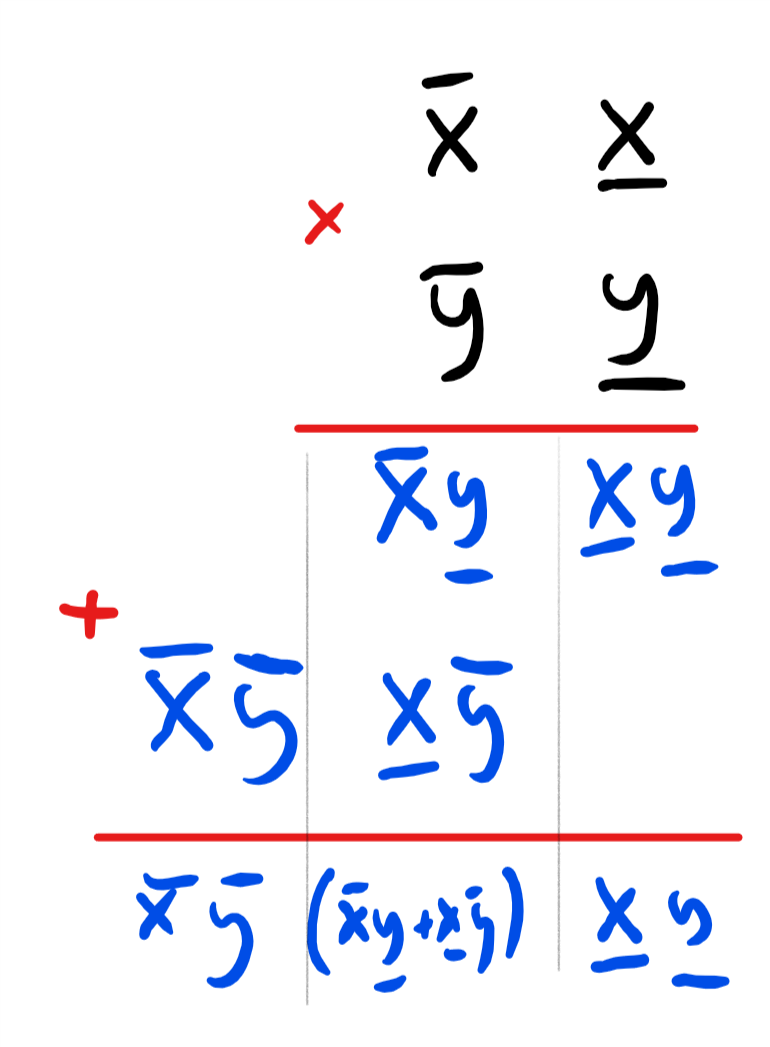
\includegraphics[width=\linewidth, height=1.5in, keepaspectratio]{../figure/gradeschoolmult.png}
\caption{The grade-school multiplication algorithm illustrated for
multiplying \(x=10\overline{x}+\underline{x}\) and
\(y=10\overline{y}+\underline{y}\). It uses the formula
\((10\overline{x}+\underline{x}) \times (10 \overline{y}+\underline{y}) = 100\overline{x}\overline{y}+10(\overline{x}\underline{y} + \underline{x}\overline{y}) + \underline{x}\underline{y}\).}
\label{gradeschoolmult}
\end{marginfigure}

The grade-school algorithm can be thought of as transforming the task of
multiplying a pair of two-digit numbers into \emph{four} single-digit
multiplications via the formula

\[
(10\overline{x}+\underline{x}) \times (10 \overline{y}+\underline{y}) = 100\overline{x}\overline{y}+10(\overline{x}\underline{y} + \underline{x}\overline{y}) + \underline{x}\underline{y} \label{eq:gradeschooltwodigit}
\]

Generally, in the grade-school algorithm \emph{doubling} the number of
digits in the input results in \emph{quadrupling} the number of
operations, leading to an \(O(n^2)\) times algorithm. In contrast,
Karatsuba's algorithm is based on the observation that we can express
\cref{eq:gradeschooltwodigit} also as

\[
(10\overline{x}+\underline{x}) \times (10 \overline{y}+\underline{y}) = (100-10)\overline{x}\overline{y}+10\left[(\overline{x}+\underline{x})(\overline{y}+\underline{y})\right]  -(10-1)\underline{x}\underline{y} \label{eq:karatsubatwodigit}
\]

which reduces multiplying the two-digit number \(x\) and \(y\) to
computing the following three simpler products:
\(\overline{x}\overline{y}\), \(\underline{x}\underline{y}\) and
\((\overline{x}+\underline{x})(\overline{y}+\underline{y})\). By
repeating the same strategy recursively, we can reduce the task of
multiplying two \(n\)-digit numbers to the task of multiplying
\emph{three} pairs of \(\floor{n/2}+1\) digit numbers.\footnote{If \(x\)
  is a number then \(\floor{x}\) is the integer obtained by rounding it
  down, see \cref{notationsec}.} Since every time we \emph{double} the
number of digits we \emph{triple} the number of operations, we will be
able to multiply numbers of \(n=2^\ell\) digits using about
\(3^\ell = n^{\log_2 3} \sim n^{1.585}\) operations.

The above is the intuitive idea behind Karatsuba's algorithm, but is not
enough to fully specify it. A complete description of an algorithm
entails a \emph{precise specification} of its operations together with
its \emph{analysis}: proof that the algorithm does in fact do what it's
supposed to do. The operations of Karatsuba's algorithm are detailed in
\cref{karatsubaalg}, while the analysis is given in
\cref{karatsubacorrect} and \cref{karatsubaefficient}.


\begin{marginfigure}
\centering
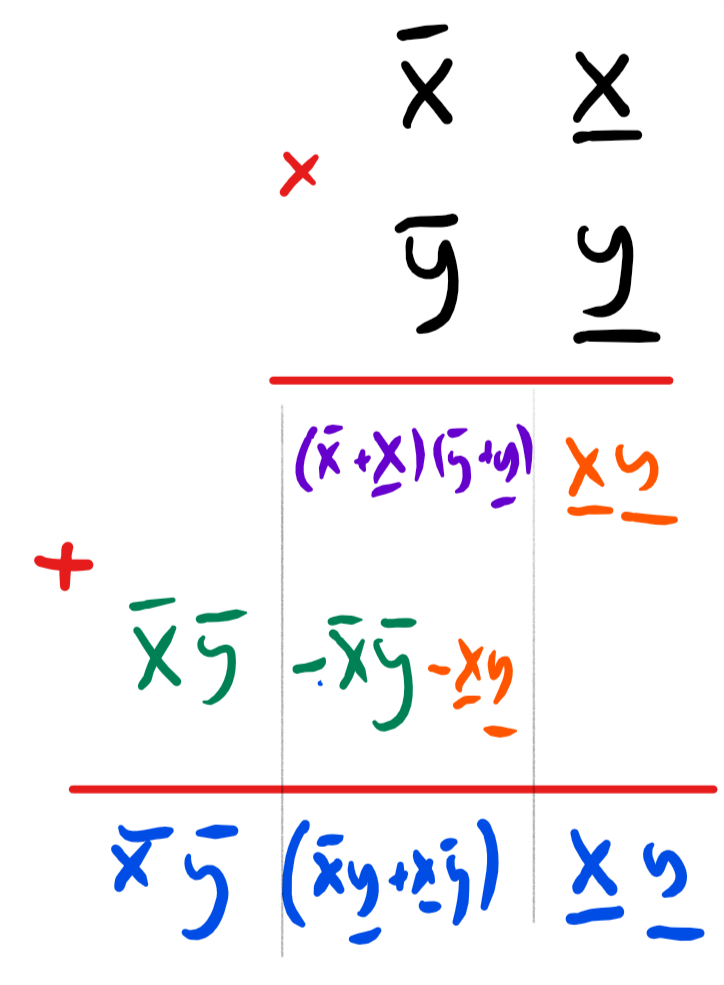
\includegraphics[width=\linewidth, height=1.5in, keepaspectratio]{../figure/karatsubatwodigit.png}
\caption{Karatsuba's multiplication algorithm illustrated for
multiplying \(x=10\overline{x}+\underline{x}\) and
\(y=10\overline{y}+\underline{y}\). We compute the three orange, green
and purple products \(\underline{x}\underline{y}\),
\(\overline{x}\overline{y}\) and
\((\overline{x}+\underline{x})(\overline{y}+\underline{y})\) and then
add and subtract them to obtain the result.}
\label{karatsubafig}
\end{marginfigure}


\begin{marginfigure}
\centering
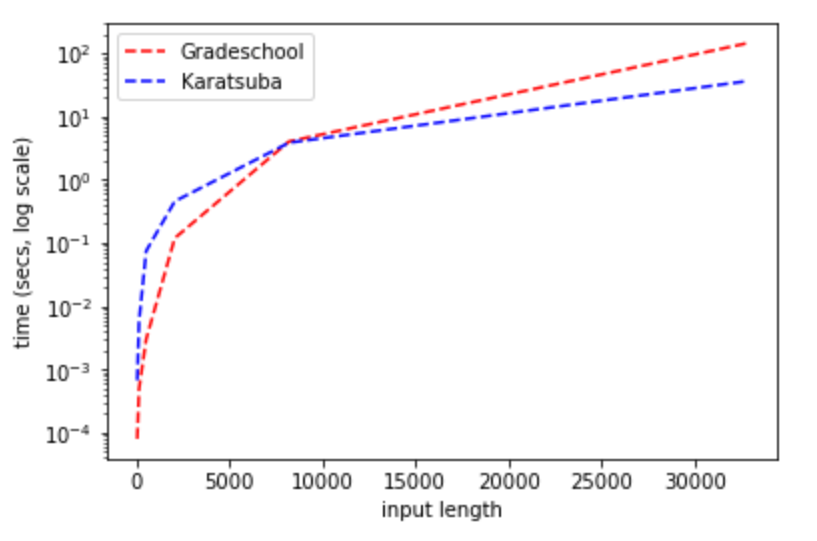
\includegraphics[width=\linewidth, height=1.5in, keepaspectratio]{../figure/karastubavsgschoolv2.png}
\caption{Running time of Karatsuba's algorithm vs.~the grade-school
algorithm. (Python implementation available
\href{https://goo.gl/zwzpYe}{online}.) Note the existence of a
``cutoff'' length, where for sufficiently large inputs Karatsuba becomes
more efficient than the grade-school algorithm. The precise cutoff
location varies by implementation and platform details, but will always
occur eventually.}
\label{karatsubaruntimefig}
\end{marginfigure}

\begin{algorithm}[Karatsuba multiplication]
\label[algorithm]{karatsubaalg} ~ \\ \noindent
\begin{algorithmic}[1]
\INPUT  nonnegative integers $x,y$ each of at most $n$ digits
\OUTPUT  $x\cdot y$
\PROCEDURE{Karatsuba}{$x$,$y$}
\IF {$n \leq 2$} \RETURN $x\cdot y$ \ENDIF
\STATE Let $m = \lfloor n/2 \rfloor$
\STATE Write $x= 10^{m}\overline{x} + \underline{x}$ and $y= 10^{m}\overline{y}+ \underline{y}$
\STATE $A \leftarrow$ \CALL{Karatsuba}{$\overline{x},\overline{y}$} 
\STATE $B \leftarrow$ \CALL{Karatsuba}{$\overline{x}+\underline{x},\overline{y}+\underline{y}$} 
\STATE $C \leftarrow$ \CALL{Karatsuba}{$\underline{x},\underline{y}$} 
\RETURN $(10^n-10^m)\cdot A  + 10^m \cdot B +(1-10^m)\cdot C$
\ENDPROCEDURE
\end{algorithmic}
\end{algorithm}

\cref{karatsubaalg} is only half of the full description of Karatsuba's
algorithm. The other half is the \emph{analysis}, which entails proving
that \textbf{(1)} \cref{karatsubaalg} indeed computes the multiplication
operation and \textbf{(2)} it does so using \(O(n^{\log_2 3})\)
operations. We now turn to showing both facts:

\hypertarget{karatsubacorrect}{}
\begin{lemma} \label[lemma]{karatsubacorrect}

For every nonnegative integers \(x,y\), when given input \(x,y\)
\cref{karatsubaalg} will output \(x\cdot y\).

\end{lemma}

\begin{proof} \label[proof]{Let-n-be-the-maximum-numb}

Let \(n\) be the maximum number of digits of \(x\) and \(y\). We prove
the lemma by induction on \(n\). The base case is \(n \leq 2\) where the
algorithm returns \(x\cdot y\) by definition. Otherwise, if \(n>2\), we
define \(m = \floor{n/2}\), and write
\(x= 10^{m}\overline{x} + \underline{x}\) and
\(y= 10^{m}\overline{y}+ \underline{y}\).

Plugging this into \(x\cdot y\), we get

\[
x \cdot y = 10^{2m} \overline{x}\overline{y} + 10^{m}(\overline{x}\underline{y} +\underline{x}\overline{y}) + \underline{x}\underline{y}  \;. \label{eqkarastubaone}
\]

Rearranging the terms we see that

\[
x\cdot y =   10^{2m}\overline{x}\overline{y} + 10^{m}\left[ (\overline{x}+\underline{x})(\overline{y}+\underline{y}) - \underline{x}\underline{y}  - \overline{x}\overline{y} \right]  + \underline{x}\underline{y} \;.
 \label{eqkarastubatwo}
\] since the numbers \(\underline{x}\),\(\overline{x}\),
\(\underline{y}\),\(\overline{y}\),\(\overline{x}+\underline{x}\),\(\overline{y}+\underline{y}\)
all have at most \(m+1<n\) digits, the induction hypothesis implies that
the values \(A,B,C\) computed by the recursive calls will satisfy
\(A=\overline{x}\overline{y}\),
\(B=(\overline{x}+\underline{x})(\overline{y}+\underline{y})\) and
\(C=\underline{x}\underline{y}\). Plugging this into
\eqref{eqkarastubatwo} we see that \(x\cdot y\) equals the value
\((10^{2m}-10^m)\cdot A + 10^m \cdot B +(1-10^m)\cdot C\) computed by
\cref{karatsubaalg}.

\end{proof}

\hypertarget{karatsubaefficient}{}
\begin{lemma} \label[lemma]{karatsubaefficient}

If \(x,y\) are integers of at most \(n\) digits, \cref{karatsubaalg}
will take \(O(n^{\log_2 3})\) operations on input \(x,y\).

\end{lemma}

\begin{proof} \label[proof]{crefkaratsubafig-illustra}

\cref{karatsubafig} illustrates the idea behind the proof, which we only
sketch here, leaving filling out the details as \cref{karatsuba-ex}. The
proof is again by induction. We define \(T(n)\) to be the maximum number
of steps that \cref{karatsubaalg} takes on inputs of length at most
\(n\). Since in the base case \(n\leq 2\), \cref{karatsuba-ex} performs
a constant number of computation, we know that \(T(2) \leq c\) for some
constant \(c\) and for \(n>2\), it satisfies the recursive equation \[
T(n) \leq 3T(\floor{n/2}+1) + c' n \label{eqkaratsubarecursion}
\] for some constant \(c'\) (using the fact that addition can be done in
\(O(n)\) operations).

The recursive equation \eqref{eqkaratsubarecursion} solves to
\(O(n^{\log_3 2})\). The intuition behind this is presented in
\cref{karatsubafig}, and this is also a consequence of the so called
\href{https://en.wikipedia.org/wiki/Master_theorem_(analysis_of_algorithms)}{``Master
Theorem''} on recurrence relations that is covered in many discrete math
texts. As mentioned above, we leave completing the proof to the reader
as \cref{karatsuba-ex}.

\end{proof}


\begin{figure}
\centering
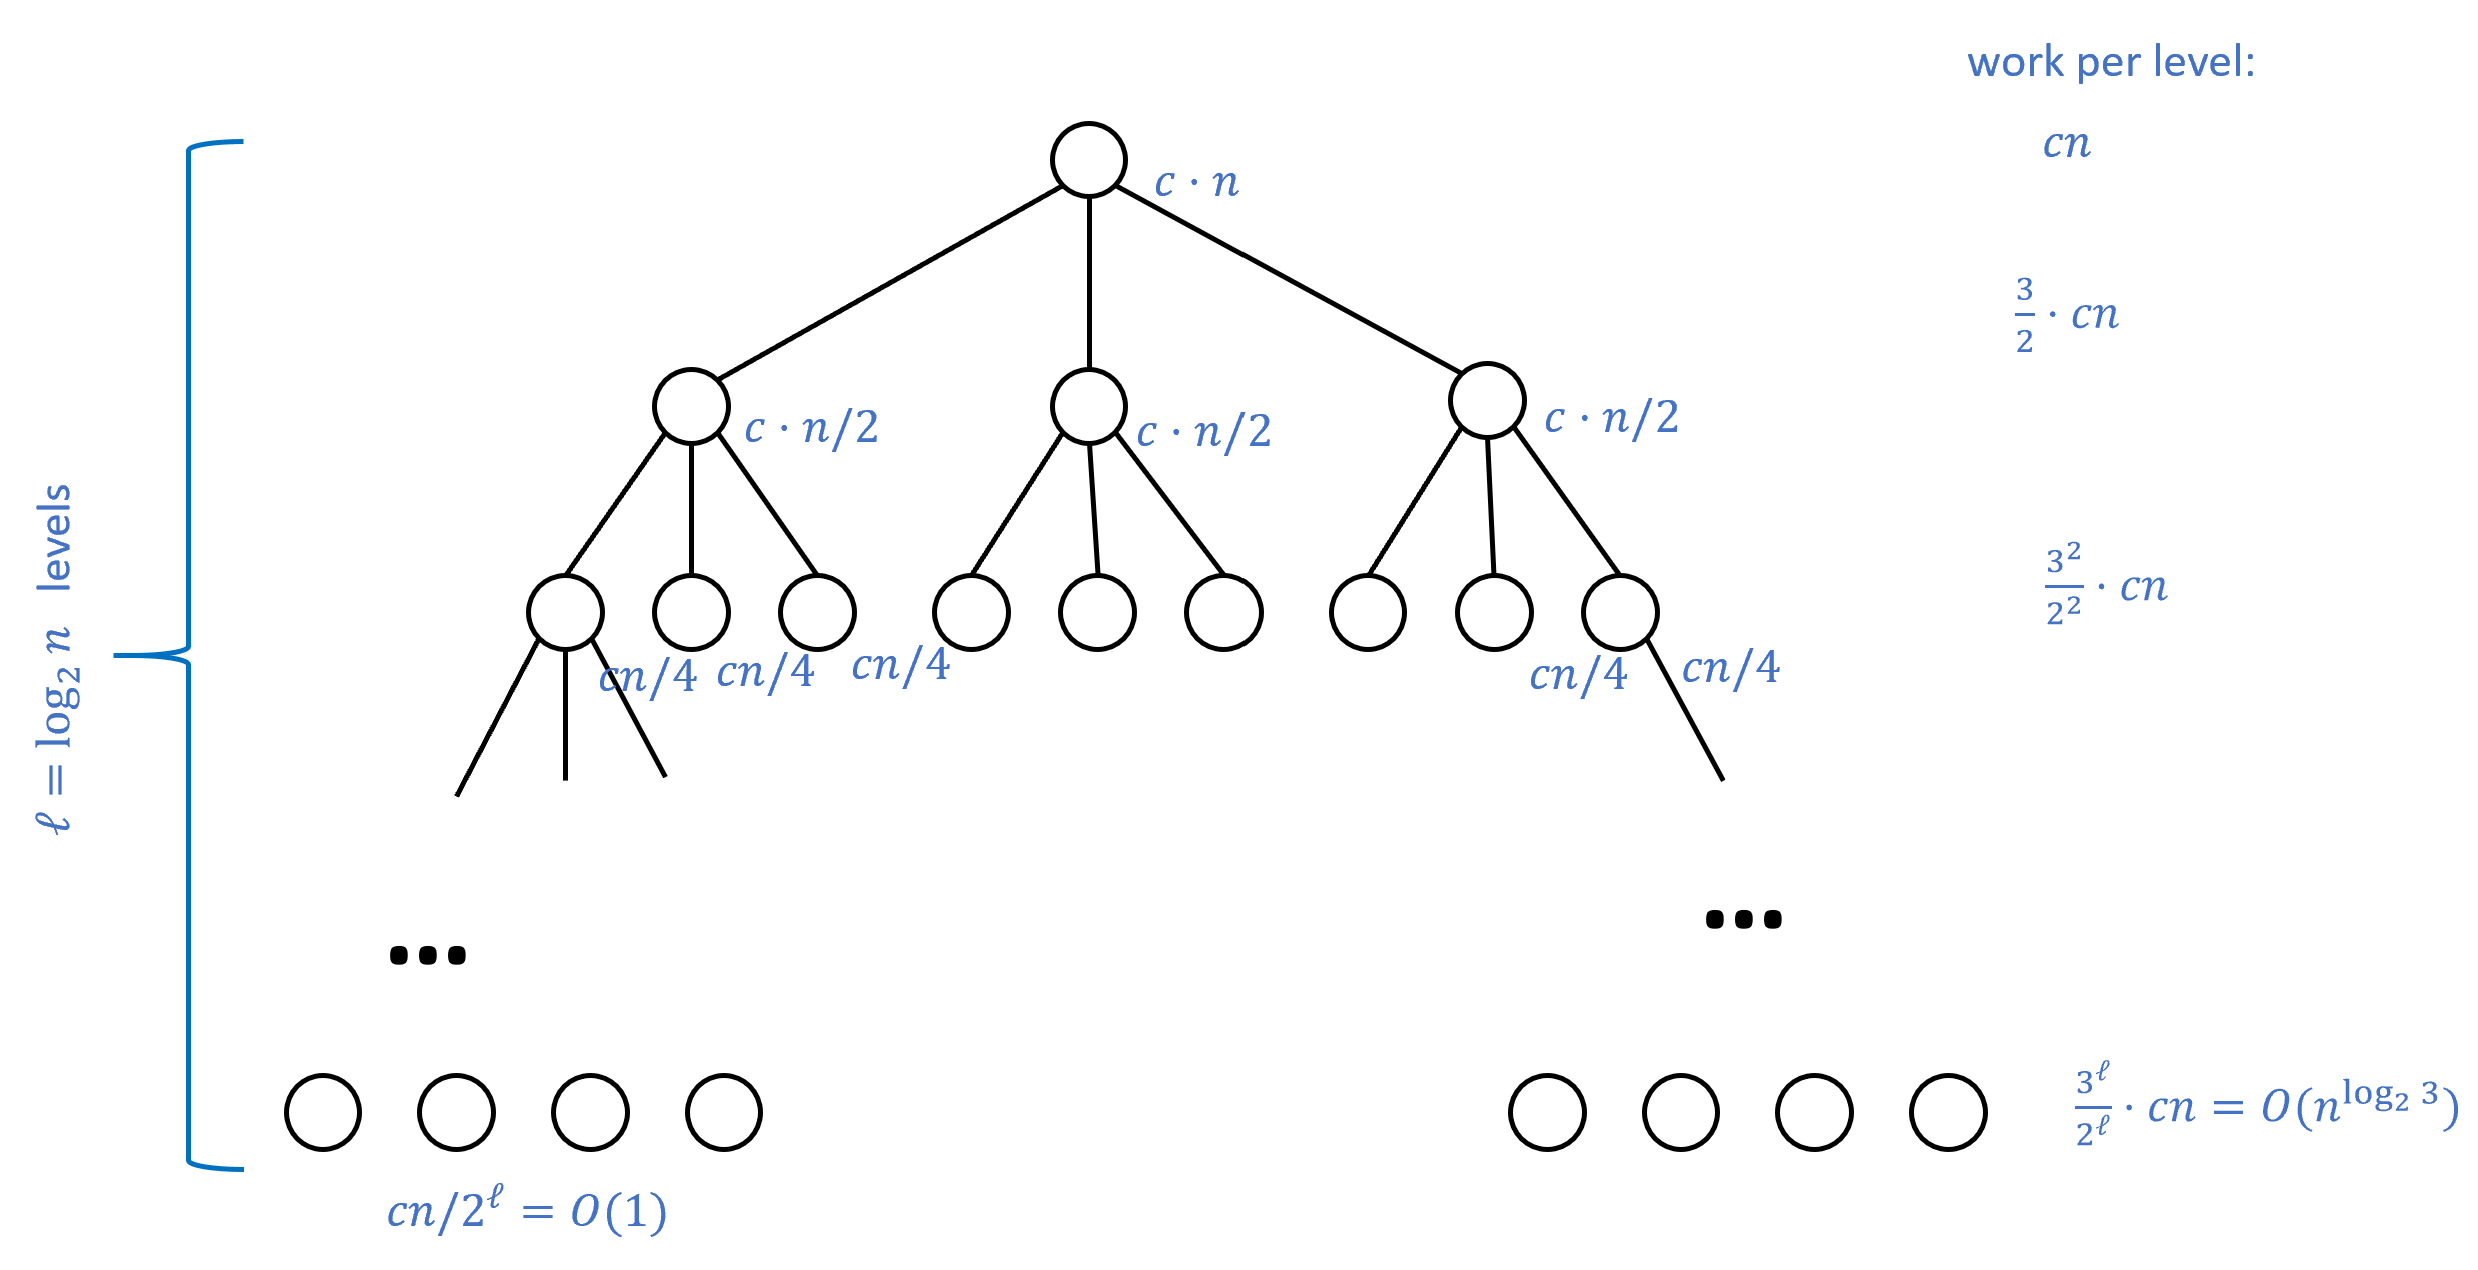
\includegraphics[width=\textwidth, height=0.25\paperheight, keepaspectratio]{../figure/karatsuba_analysis2.png}
\caption{Karatsuba's algorithm reduces an \(n\)-bit multiplication to
three \(n/2\)-bit multiplications, which in turn are reduced to nine
\(n/4\)-bit multiplications and so on. We can represent the
computational cost of all these multiplications in a \(3\)-ary tree of
depth \(\log_2 n\), where at the root the extra cost is \(cn\)
operations, at the first level the extra cost is \(c(n/2)\) operations,
and at each of the \(3^i\) nodes of level \(i\), the extra cost is
\(c(n/2^i)\). The total cost is
\(cn\sum_{i=0}^{\log_2 n} (3/2)^i \leq 10cn^{\log_2 3}\) by the formula
for summing a geometric series.}
\label{karatsuba-fig}
\end{figure}

Karatsuba's algorithm is by no means the end of the line for
multiplication algorithms. In the 1960's, Toom and Cook extended
Karatsuba's ideas to get an \(O(n^{\log_k (2k-1)})\) time multiplication
algorithm for every constant \(k\). In 1971, Schönhage and Strassen got
even better algorithms using the \emph{Fast Fourier Transform}; their
idea was to somehow treat integers as ``signals'' and do the
multiplication more efficiently by moving to the Fourier domain. (The
\emph{Fourier transform} is a central tool in mathematics and
engineering, used in a great many applications; if you have not seen it
yet, you are likely encounter it at some point in your studies.) In the
years that followed researchers kept improving the algorithm, and only
very recently Harvey and Van Der Hoeven managed to obtain an
\(O(n \log n)\) time algorithm for multiplication (though it only starts
beating the Schönhage-Strassen algorithm for truly astronomical
numbers). Yet, despite all this progress, we still don't know whether or
not there is an \(O(n)\) time algorithm for multiplying two \(n\) digit
numbers!

\hypertarget{matrixmult}{}
\begin{remark}[Matrix Multiplication (advanced note)] \label[remark]{matrixmult}

(This book contains many ``advanced'' or ``optional'' notes and
sections. These may assume background that not every student has, and
can be safely skipped over as none of the future parts depends on them.)

Ideas similar to Karatsuba's can be used to speed up \emph{matrix}
multiplications as well. Matrices are a powerful way to represent linear
equations and operations, widely used in a great many applications of
scientific computing, graphics, machine learning, and many many more.

One of the basic operations one can do with two matrices is to
\emph{multiply} them. For example, if
\(x = \begin{pmatrix} x_{0,0} & x_{0,1}\\ x_{1,0}& x_{1,1} \end{pmatrix}\)
and
\(y = \begin{pmatrix} y_{0,0} & y_{0,1}\\ y_{1,0}& y_{1,1} \end{pmatrix}\)
then the product of \(x\) and \(y\) is the matrix
\(\begin{pmatrix} x_{0,0}y_{0,0} + x_{0,1}y_{1,0} & x_{0,0}y_{0,1} + x_{0,1}y_{1,1}\\ x_{1,0}y_{0,0}+x_{1,1}y_{1,0} & x_{1,0}y_{0,1}+x_{1,1}y_{1,1} \end{pmatrix}\).
You can see that we can compute this matrix by \emph{eight} products of
numbers.

Now suppose that \(n\) is even and \(x\) and \(y\) are a pair of
\(n\times n\) matrices which we can think of as each composed of four
\((n/2)\times (n/2)\) blocks \(x_{0,0},x_{0,1},x_{1,0},x_{1,1}\) and
\(y_{0,0},y_{0,1},y_{1,0},y_{1,1}\). Then the formula for the matrix
product of \(x\) and \(y\) can be expressed in the same way as above,
just replacing products \(x_{a,b}y_{c,d}\) with \emph{matrix} products,
and addition with matrix addition. This means that we can use the
formula above to give an algorithm that \emph{doubles} the dimension of
the matrices at the expense of increasing the number of operation by a
factor of \(8\), which for \(n=2^\ell\) results in \(8^\ell = n^3\)
operations.

In 1969 Volker Strassen noted that we can compute the product of a pair
of two-by-two matrices using only \emph{seven} products of numbers by
observing that each entry of the matrix \(xy\) can be computed by adding
and subtracting the following seven terms:
\(t_1 = (x_{0,0}+x_{1,1})(y_{0,0}+y_{1,1})\),
\(t_2 = (x_{0,0}+x_{1,1})y_{0,0}\), \(t_3 = x_{0,0}(y_{0,1}-y_{1,1})\),
\(t_4 = x_{1,1}(y_{0,1}-y_{0,0})\), \(t_5 = (x_{0,0}+x_{0,1})y_{1,1}\),
\(t_6 = (x_{1,0}-x_{0,0})(y_{0,0}+y_{0,1})\),
\(t_7 = (x_{0,1}-x_{1,1})(y_{1,0}+y_{1,1})\). Indeed, one can verify
that
\(xy = \begin{pmatrix} t_1 + t_4 - t_5 + t_7 & t_3 + t_5 \\ t_2 +t_4 & t_1 + t_3 - t_2 + t_6 \end{pmatrix}\).

Using this observation, we can obtain an algorithm such that doubling
the dimension of the matrices results in increasing the number of
operations by a factor of \(7\), which means that for \(n=2^\ell\) the
cost is \(7^\ell = n^{\log_2 7} \sim n^{2.807}\). A long sequence of
work has since improved this algorithm, and the
\href{https://en.wikipedia.org/wiki/Matrix_multiplication_algorithm\#Sub-cubic_algorithms}{current
record} has running time about \(O(n^{2.373})\). However, unlike the
case of integer multiplication, at the moment we don't know of any
algorithm for matrix multiplication that runs in time linear or even
close to linear in the size of the input matrices (e.g., an
\(O(n^2 polylog(n))\) time algorithm). People have tried to use
\href{https://en.wikipedia.org/wiki/Group_representation}{group
representations}, which can be thought of as generalizations of the
Fourier transform, to obtain faster algorithms, but this effort
\href{http://discreteanalysisjournal.com/article/1245-on-cap-sets-and-the-group-theoretic-approach-to-matrix-multiplication}{has
not yet succeeded}.

\end{remark}

\section{Algorithms beyond arithmetic}\label{algsbeyondarithmetic}

The quest for better algorithms is by no means restricted to arithmetic
tasks such as adding, multiplying or solving equations. Many \emph{graph
algorithms}, including algorithms for finding paths, matchings, spanning
trees, cuts, and flows, have been discovered in the last several
decades, and this is still an intensive area of research. (For example,
the last few years saw many advances in algorithms for the \emph{maximum
flow} problem, borne out of unexpected connections with electrical
circuits and linear equation solvers.) These algorithms are being used
not just for the ``natural'' applications of routing network traffic or
GPS-based navigation, but also for applications as varied as drug
discovery through searching for structures in gene-interaction graphs to
computing risks from correlations in financial investments.

Google was founded based on the \emph{PageRank} algorithm, which is an
efficient algorithm to approximate the ``principal eigenvector'' of (a
dampened version of) the adjacency matrix of the web graph. The
\emph{Akamai} company was founded based on a new data structure, known
as \emph{consistent hashing}, for a hash table where buckets are stored
at different servers. The \emph{backpropagation algorithm}, which
computes partial derivatives of a neural network in \(O(n)\) instead of
\(O(n^2)\) time, underlies many of the recent phenomenal successes of
learning deep neural networks. Algorithms for solving linear equations
under sparsity constraints, a concept known as \emph{compressed
sensing}, have been used to drastically reduce the amount and quality of
data needed to analyze MRI images. This made a critical difference for
MRI imaging of cancer tumors in children, where previously doctors
needed to use anesthesia to suspend breath during the MRI exam,
sometimes with dire consequences.

Even for classical questions, studied through the ages, new discoveries
are still being made. For example, for the question of determining
whether a given integer is prime or composite, which has been studied
since the days of Pythagoras, efficient probabilistic algorithms were
only discovered in the 1970s, while the first
\href{https://en.wikipedia.org/wiki/AKS_primality_test}{deterministic
polynomial-time algorithm} was only found in 2002. For the related
problem of actually finding the factors of a composite number, new
algorithms were found in the 1980s, and (as we'll see later in this
course) discoveries in the 1990s raised the tantalizing prospect of
obtaining faster algorithms through the use of quantum mechanical
effects.

Despite all this progress, there are still many more questions than
answers in the world of algorithms. For almost all natural problems, we
do not know whether the current algorithm is the ``best'', or whether a
significantly better one is still waiting to be discovered. As alluded
in Cobham's opening quote for this chapter, even for the basic problem
of multiplying numbers we have not yet answered the question of whether
there is a multiplication algorithm that is as efficient as our
algorithms for addition. But at least we now know the right way to
\emph{ask} it.

\section{On the importance of negative
results.}\label{On-the-importance-of-nega}

Finding better algorithms for problems such as multiplication, solving
equations, graph problems, or fitting neural networks to data, is
undoubtedly a worthwhile endeavor. But why is it important to prove that
such algorithms \emph{don't} exist? One motivation is pure intellectual
curiosity. Another reason to study impossibility results is that they
correspond to the fundamental limits of our world. In other words,
impossibility results are \emph{laws of nature}.

Here are some examples of impossibility results outside computer science
(see \cref{bnotesintrosec} for more about these). In physics, the
impossibility of building a \emph{perpetual motion machine} corresponds
to the \emph{law of conservation of energy}. The impossibility of
building a heat engine beating Carnot's bound corresponds to the second
law of thermodynamics, while the impossibility of faster-than-light
information transmission is a cornerstone of special relativity. In
mathematics, while we all learned the formula for solving quadratic
equations in high school, the impossibility of generalizing this formula
to equations of degree five or more gave birth to \emph{group theory}.
The impossibility of proving Euclid's fifth axiom from the first four
gave rise to \emph{non-Euclidean geometries}, which ended up crucial for
the theory of general relativity.

In an analogous way, impossibility results for computation correspond to
``computational laws of nature'' that tell us about the fundamental
limits of any information processing apparatus, whether based on
silicon, neurons, or quantum particles. Moreover, computer scientists
found creative approaches to \emph{apply} computational limitations to
achieve certain useful tasks. For example, much of modern Internet
traffic is encrypted using the
\href{https://en.wikipedia.org/wiki/RSA_(cryptosystem)}{RSA encryption
scheme}, which relies on its security on the (conjectured) impossibility
of efficiently factoring large integers. More recently, the
\href{https://en.wikipedia.org/wiki/Bitcoin}{Bitcoin} system uses a
digital analog of the ``gold standard'' where, instead of using a
precious metal, new currency is obtained by ``mining'' solutions for
computationally difficult problems.

\begin{recap} \label[recap]{The-history-of-algorithms}

\begin{itemize}
\tightlist
\item
  The history of algorithms goes back thousands of years; they have been
  essential much of human progress and these days form the basis of
  multi-billion dollar industries, as well as life-saving technologies.
\item
  There is often more than one algorithm to achieve the same
  computational task. Finding a faster algorithm can often make a much
  bigger difference than improving computing hardware.
\item
  Better algorithms and data structures don't just speed up
  calculations, but can yield new qualitative insights.
\item
  One question we will study is to find out what is the \emph{most
  efficient} algorithm for a given problem.
\item
  To show that an algorithm is the most efficient one for a given
  problem, we need to be able to \emph{prove} that it is
  \emph{impossible} to solve the problem using a smaller amount of
  computational resources.
\end{itemize}

\end{recap}

\section{Roadmap to the rest of this book}\label{roadmapsec}

Often, when we try to solve a computational problem, whether it is
solving a system of linear equations, finding the top eigenvector of a
matrix, or trying to rank Internet search results, it is enough to use
the ``I know it when I see it'' standard for describing algorithms. As
long as we find some way to solve the problem, we are happy and might
not care much on the exact mathematical model for our algorithm. But
when we want to answer a question such as ``does there \emph{exist} an
algorithm to solve the problem \(P\)?'' we need to be much more precise.

In particular, we will need to \textbf{(1)} define exactly what it means
to solve \(P\), and \textbf{(2)} define exactly what an algorithm is.
Even \textbf{(1)} can sometimes be non-trivial but \textbf{(2)} is
particularly challenging; it is not at all clear how (and even whether)
we can encompass all potential ways to design algorithms. We will
consider several simple \emph{models of computation}, and argue that,
despite their simplicity, they do capture all ``reasonable'' approaches
to achieve computing, including all those that are currently used in
modern computing devices.

Once we have these formal models of computation, we can try to obtain
\emph{impossibility results} for computational tasks, showing that some
problems \emph{can not be solved} (or perhaps can not be solved within
the resources of our universe). Archimedes once said that given a
fulcrum and a long enough lever, he could move the world. We will see
how \emph{reductions} allow us to leverage one hardness result into a
slew of a great many others, illuminating the boundaries between the
computable and uncomputable (or tractable and intractable) problems.

Later in this book we will go back to examining our models of
computation, and see how resources such as randomness or quantum
entanglement could potentially change the power of our model. In the
context of probabilistic algorithms, we will see a glimpse of how
randomness has become an indispensable tool for understanding
computation, information, and communication. We will also see how
computational difficulty can be an asset rather than a hindrance, and be
used for the ``derandomization'' of probabilistic algorithms. The same
ideas also show up in \emph{cryptography}, which has undergone not just
a technological but also an intellectual revolution in the last few
decades, much of it building on the foundations that we explore in this
course.

Theoretical Computer Science is a vast topic, branching out and touching
upon many scientific and engineering disciplines. This book provides a
very partial (and biased) sample of this area. More than anything, I
hope I will manage to ``infect'' you with at least some of my love for
this field, which is inspired and enriched by the connection to
practice, but is also deep and beautiful regardless of applications.

\subsection{Dependencies between
chapters}\label{Dependencies-between-chap}

This book is divided into the following parts, see
\cref{dependencystructurefig}.

\begin{itemize}
\item
  \textbf{Preliminaries:} Introduction, mathematical background, and
  representing objects as strings.
\item
  \textbf{Part I: Finite computation (Boolean circuits):} Equivalence of
  circuits and straight-line programs. Universal gate sets. Existence of
  a circuit for every function, representing circuits as strings,
  universal circuit, lower bound on circuit size using the counting
  argument.
\item
  \textbf{Part II: Uniform computation (Turing machines):} Equivalence
  of Turing machines and programs with loops. Equivalence of models
  (including RAM machines, \(\lambda\) calculus, and cellular automata),
  configurations of Turing machines, existence of a universal Turing
  machine, uncomputable functions (including the Halting problem and
  Rice's Theorem), Gödel's incompleteness theorem, restricted
  computational models models (regular and context free languages).
\item
  \textbf{Part III: Efficient computation:} Definition of running time,
  time hierarchy theorem, \(\mathbf{P}\) and \(\mathbf{NP}\),
  \(\mathbf{P_{/poly}}\), \(\mathbf{NP}\) completeness and the
  Cook-Levin Theorem, space bounded computation.
\item
  \textbf{Part IV: Randomized computation:} Probability, randomized
  algorithms, \(\mathbf{BPP}\), amplification,
  \(\mathbf{BPP} \subseteq \mathbf{P}_{/poly}\), pseudorandom generators
  and derandomization.
\item
  \textbf{Part V: Advanced topics:} Cryptography, proofs and algorithms
  (interactive and zero knowledge proofs, Curry-Howard correspondence),
  quantum computing.
\end{itemize}


\begin{figure}
\centering
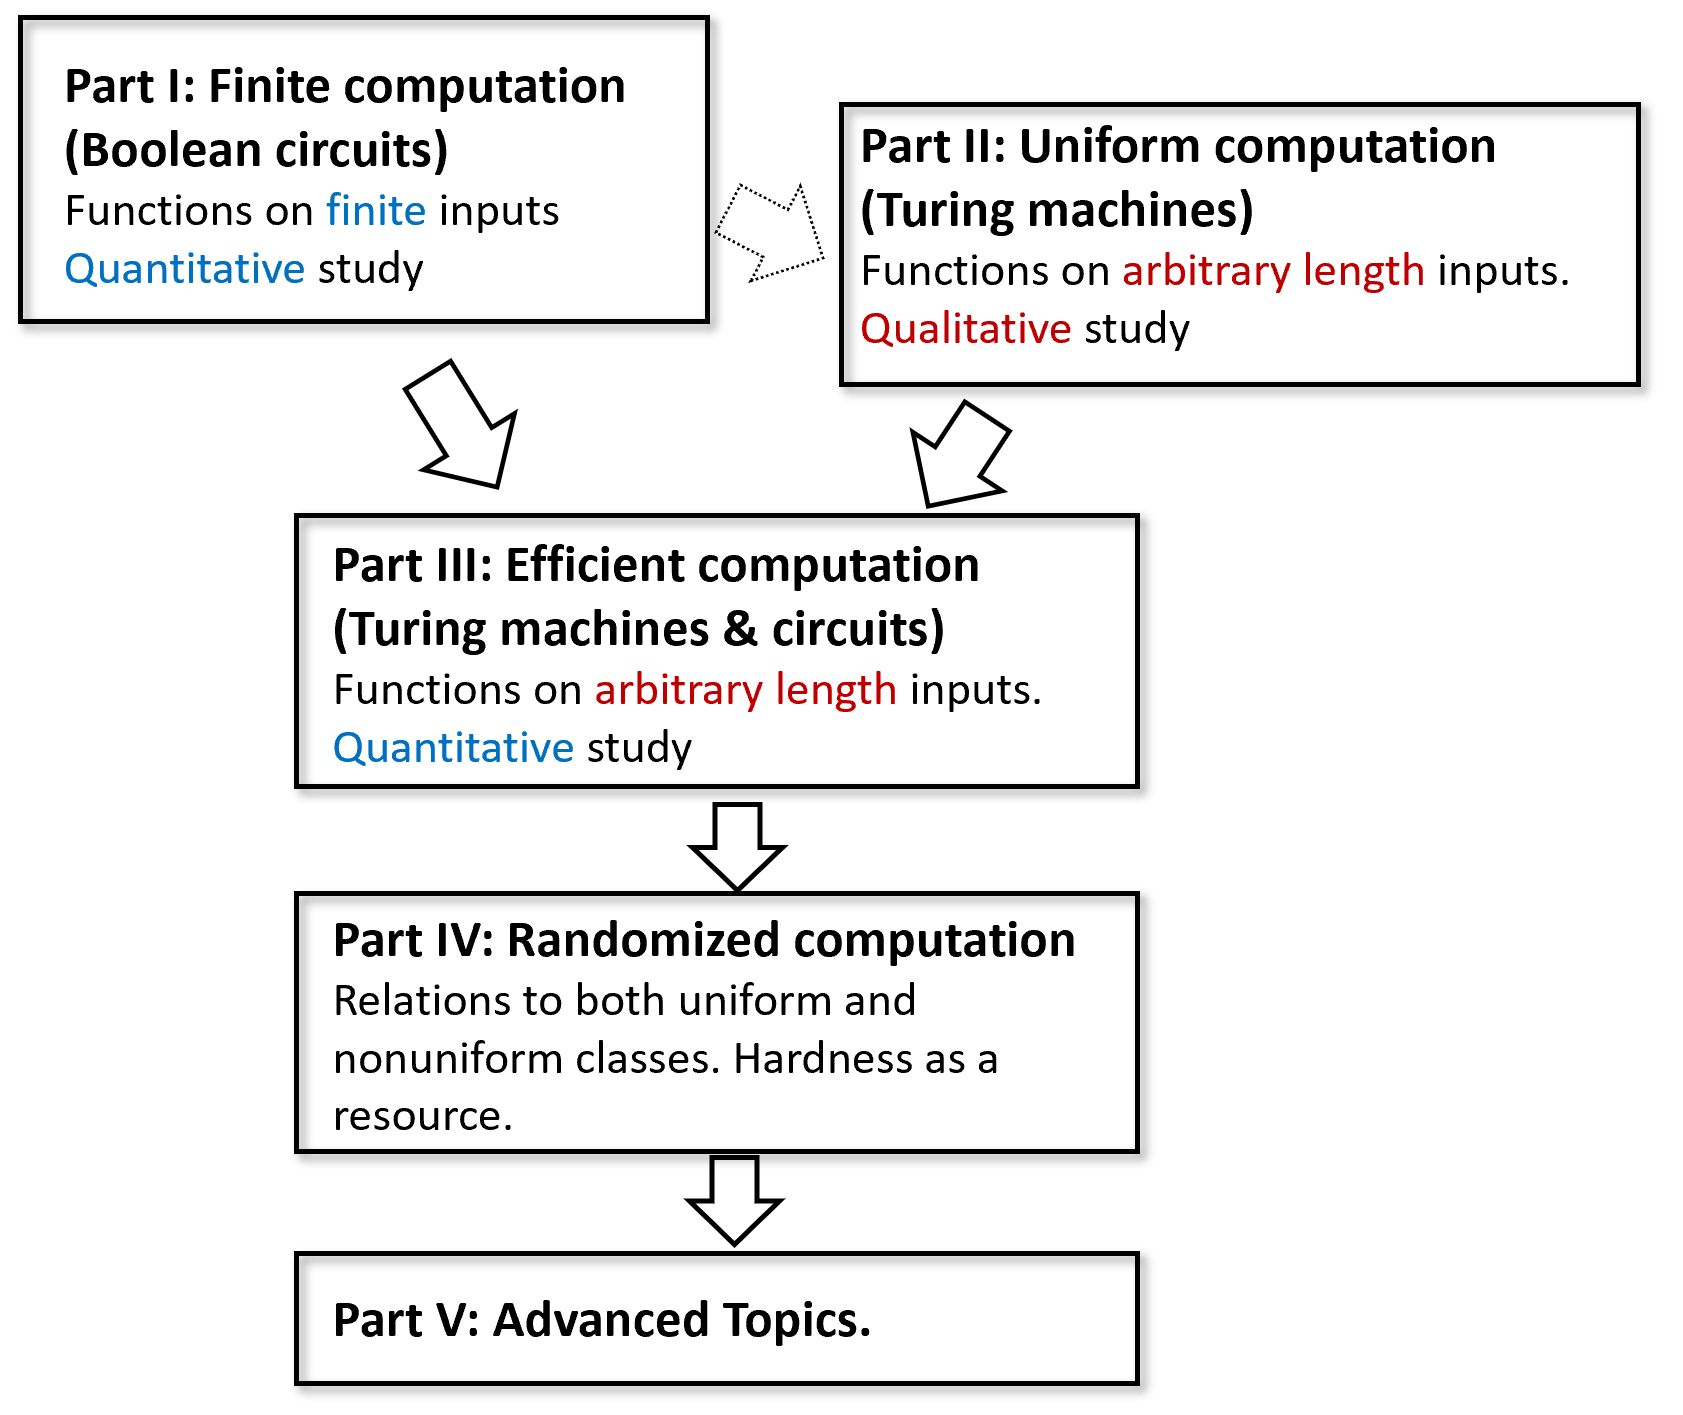
\includegraphics[width=\textwidth, height=0.25\paperheight, keepaspectratio]{../figure/dependencystructure.png}
\caption{The dependency structure of the different parts. Part I
introduces the model of Boolean circuits to study \emph{finite
functions} with an emphasis on \emph{quantitative} questions (how many
gates to compute a function). Part II introduces the model of Turing
machines to study functions that have \emph{unbounded input lengths}
with an emphasis on \emph{qualitative} questions (is this function
computable or not). Much of Part II does not depend on Part I, as Turing
machines can be used as the first computational model. Part III depends
on both parts as it introduces a \emph{quantitative} study of functions
with unbounded input length. The more advancec parts IV (randomized
computation) and V (advanced topics) rely on the material of Parts I, II
and III.}
\label{dependencystructurefig}
\end{figure}

The book largely proceeds in linear order, with each chapter building on
the previous ones, with the following exceptions:

\begin{itemize}
\item
  The topics of \(\lambda\) calculus (\cref{lambdacalculussec} and
  \cref{lambdacalculussec}), Gödel's incompleteness theorem
  (\cref{godelchap}), Automata/regular expressions and context-free
  grammars (\cref{restrictedchap}), and space-bounded computation
  (\cref{spacechap}), are not used in the following chapters. Hence you
  can choose whether to cover or skip any subset of them.
\item
  Part II (Uniform Computation / Turing Machines) does not have a strong
  dependency on Part I (Finite computation / Boolean circuits) and it
  should be possible to teach them in the reverse order with minor
  modification. Boolean circuits are used Part III (efficient
  computation) for results such as
  \(\mathbf{P} \subseteq \mathbf{P_{/poly}}\) and the Cook-Levin
  Theorem, as well as in Part IV (for
  \(\mathbf{BPP} \subseteq \mathbf{P_{/poly}}\) and derandomization) and
  Part V (specifically in cryptography and quantum computing).
\item
  All chapters in \cref{advancedpart} (Advanced topics) are independent
  of one another and can be covered in any order.
\end{itemize}

A course based on this book can use all of Parts I, II, and III
(possibly skipping over some or all of the \(\lambda\) calculus,
\cref{godelchap}, \cref{restrictedchap} or \cref{spacechap}), and then
either cover all or some of Part IV (randomized computation), and add a
``sprinkling'' of advanced topics from Part V based on student or
instructor interest.

\section{Exercises}\label{Exercises}

\begin{exercise} \label[exercise]{Rank-the-significance-of-}

Rank the significance of the following inventions in speeding up
multiplication of large (that is 100-digit or more) numbers. That is,
use ``back of the envelope'' estimates to order them in terms of the
speedup factor they offered over the previous state of affairs.

\begin{enumerate}
\def\labelenumi{\alph{enumi}.}
\item
  Discovery of the grade-school digit by digit algorithm (improving upon
  repeated addition)
\item
  Discovery of Karatsuba's algorithm (improving upon the digit by digit
  algorithm)
\item
  Invention of modern electronic computers (improving upon calculations
  with pen and paper).
\end{enumerate}

\end{exercise}

\begin{exercise} \label[exercise]{The--Apple-II-personal-co}

The 1977 Apple II personal computer had a processor speed of 1.023 Mhz
or about \(10^6\) operations per seconds. At the time of this writing
the world's fastest supercomputer performs 93 ``petaflops'' (\(10^{15}\)
floating point operations per second) or about \(10^{18}\) basic steps
per second. For each one of the following running times (as a function
of the input length \(n\)), compute for both computers how large an
input they could handle in a week of computation, if they run an
algorithm that has this running time:

\begin{enumerate}
\def\labelenumi{\alph{enumi}.}
\item
  \(n\) operations.
\item
  \(n^2\) operations.
\item
  \(n\log n\) operations.
\item
  \(2^n\) operations.
\item
  \(n!\) operations.
\end{enumerate}

\end{exercise}

\begin{exercise}[Usefulness of algorithmic non-existence] \label[exercise]{In-this-chapter-we-mentio}

In this chapter we mentioned several companies that were founded based
on the discovery of new algorithms. Can you give an example for a
company that was founded based on the \emph{non existence} of an
algorithm? See footnote for hint.\footnote{As we will see in Chapter
  \cref{chapcryptography}, almost any company relying on cryptography
  needs to assume the \emph{non existence} of certain algorithms. In
  particular, \href{https://goo.gl/tMsAui}{RSA Security} was founded
  based on the security of the RSA cryptosystem, which presumes the
  \emph{non existence} of an efficient algorithm to compute the prime
  factorization of large integers.}

\end{exercise}

\hypertarget{karatsuba-ex}{}
\begin{exercise}[Analysis of Karatsuba's Algorithm] \label[exercise]{karatsuba-ex}

\begin{enumerate}
\def\labelenumi{\alph{enumi}.}
\item
  Suppose that \(T_1,T_2,T_3,\ldots\) is a sequence of numbers such that
  \(T_2 \leq 10\) and for every \(n\),
  \(T_n \leq 3T_{\lfloor n/2 \rfloor+1} + Cn\) for some \(C \geq 1\).
  Prove that \(T_n \leq 20Cn^{\log_2 3}\) for every \(n>2\).\footnote{\textbf{Hint:}
    Use a proof by induction - suppose that this is true for all \(n\)'s
    from \(1\) to \(m\) and prove that this is true also for \(m+1\).}\\
\item
  Prove that the number of single-digit operations that Karatsuba's
  algorithm takes to multiply two \(n\) digit numbers is at most
  \(1000n^{\log_2 3}\).
\end{enumerate}

\end{exercise}

\begin{exercise} \label[exercise]{Implement-in-the-programm}

Implement in the programming language of your choice functions
\texttt{Gradeschool\_multiply(x,y)} and
\texttt{Karatsuba\_multiply(x,y)} that take two arrays of digits
\texttt{x} and \texttt{y} and return an array representing the product
of \texttt{x} and \texttt{y} (where \texttt{x} is identified with the
number \texttt{x[0]+10*x[1]+100*x[2]+...} etc..) using the grade-school
algorithm and the Karatsuba algorithm respectively. At what number of
digits does the Karatsuba algorithm beat the grade-school one?

\end{exercise}

\hypertarget{matrixex}{}
\begin{exercise}[Matrix Multiplication (optional, advanced)] \label[exercise]{matrixex}

In this exercise, we show that if for some \(\omega>2\), we can write
the product of two \(k\times k\) real-valued matrices \(A,B\) using at
most \(k^\omega\) multiplications, then we can multiply two
\(n\times n\) matrices in roughly \(n^\omega\) time for every large
enough \(n\).

To make this precise, we need to make some notation that is
unfortunately somewhat cumbersome. Assume that there is some \(k\in \N\)
and \(m \leq k^\omega\) such that for every \(k\times k\) matrices
\(A,B,C\) such that \(C=\ensuremath{\mathit{AB}}\), we can write for
every \(i,j \in [k]\): \[
C_{i,j} = \sum_{\ell=0}^m \alpha_{i,j}^\ell f_\ell(A)g_\ell(B)
\] for some linear functions
\(f_0,\ldots,f_{m-1},g_0,\ldots,g_{m-1}:\mathbb{R}^{n^2} \rightarrow \mathbb{R}\)
and coefficients \(\{ \alpha_{i,j}^\ell \}_{i,j \in [k],\ell \in [m]}\).
Prove that under this assumption for every \(\epsilon>0\), if \(n\) is
sufficiently large, then there is an algorithm that computes the product
of two \(n\times n\) matrices using at most \(O(n^{\omega+\epsilon})\)
arithmetic operations. See footnote for hint.\footnote{Start by showing
  this for the case that \(n=k^t\) for some natural number \(t\), in
  which case you can do so recursively by breaking the matrices into
  \(k\times k\) blocks.}

\end{exercise}

\section{Bibliographical notes}\label{bnotesintrosec}

For a brief overview of what we'll see in this book, you could do far
worse than read
\href{https://www.cs.princeton.edu/~chazelle/pubs/algorithm.html}{Bernard
Chazelle's wonderful essay on the Algorithm as an Idiom of modern
science}. The book of Moore and Mertens \cite{MooreMertens11} gives a
wonderful and comprehensive overview of the theory of computation,
including much of the content discussed in this chapter and the rest of
this book. Aaronson's book \cite{Aaronson13democritus} is another great
read that touches upon many of the same themes.

For more on the algorithms the Babylonians used, see
\href{http://steiner.math.nthu.edu.tw/disk5/js/computer/1.pdf}{Knuth's
paper} and Neugebauer's
\href{https://www.amazon.com/Exact-Sciences-Antiquity-Neugebauer/dp/0486223329}{classic
book}.

Many of the algorithms we mention in this chapter are covered in
algorithms textbooks such as those by Cormen, Leiserson, Rivert, and
Stein \cite{CLRS}, Kleinberg and Tardos \cite{KleinbergTardos06}, and
Dasgupta, Papadimitriou and Vazirani \cite{DasguptaPV08}, as well as
\href{http://jeffe.cs.illinois.edu/teaching/algorithms/}{Jeff Erickson's
textbook}. Erickson's book is freely available online and contains a
great exposition of recursive algorithms in general and Karatsuba's
algorithm in particular.

The story of Karatsuba's discovery of his multiplication algorithm is
recounted by him in \cite{Karatsuba95}. As mentioned above, further
improvements were made by Toom and Cook \cite{Toom63, Cook66}, Schönhage
and Strassen \cite{SchonhageStrassen71}, Fürer \cite{Furer07}, and
recently by Harvey and Van Der Hoeven \cite{HarveyvdHoeven2019}, see
\href{https://www.quantamagazine.org/mathematicians-discover-the-perfect-way-to-multiply-20190411/}{this
article} for a nice overview. The last papers crucially rely on the
\emph{Fast Fourier transform} algorithm. The fascinating story of the
(re)discovery of this algorithm by John Tukey in the context of the cold
war is recounted in \cite{Cooley87FFTdiscovery}. (We say re-discovery
because it later turned out that the algorithm dates back to Gauss
\cite{heideman1985gauss}.) The Fast Fourier Transform is covered in some
of the books mentioned below, and there are also online available
lectures such as
\href{http://jeffe.cs.illinois.edu/teaching/algorithms/}{Jeff
Erickson's}. See also this
\href{http://www.ams.org/samplings/feature-column/fcarc-multiplication}{popular
article by David Austin}. Fast \emph{matrix} multiplication was
discovered by Strassen \cite{Strassen69}, and since then this has been
an active area of research. \cite{Blaser13} is a recommended
self-contained survey of this area.

The \emph{Backpropagation} algorithm for fast differentiation of neural
networks was invented by Werbos \cite{Werbos74}. The \emph{Pagerank}
algorithm was invented by Larry Page and Sergey Brin \cite{pagerank99}.
It is closely related to the \emph{HITS} algorithm of Kleinberg
\cite{Kleinber99}. The \emph{Akamai} company was founded based on the
\emph{consistent hashing} data structure described in \cite{Akamai97}.
\emph{Compressed sensing} has a long history but two foundational papers
are \cite{CandesRombergTao06, Donoho2006compressed}.
\cite{compressedmri08} gives a survey of applications of compressed
sensing to MRI; see also this popular article by Ellenberg
\cite{Ellenberg10wired}. The deterministic polynomial-time algorithm for
testing primality was given by Agrawal, Kayal, and Saxena
\cite{AgrawalKayalSaxena04}.

We alluded briefly to classical impossibility results in mathematics,
including the impossibility of proving Euclid's fifth postulate from the
other four, impossibility of trisecting an angle with a straightedge and
compass and the impossibility of solving a quintic equation via
radicals. A geometric proof of the impossibility of angle trisection
(one of the three
\href{http://mathworld.wolfram.com/GeometricProblemsofAntiquity.html}{geometric
problems of antiquity}, going back to the ancient Greeks) is given in
this
\href{https://terrytao.wordpress.com/2011/08/10/a-geometric-proof-of-the-impossibility-of-angle-trisection-by-straightedge-and-compass/}{blog
post of Tao}. The book of Mario Livio \cite{Livio05} covers some of the
background and ideas behind these impossibility results. Some
\href{http://www.scottaaronson.com/barbados-2016.pdf}{exciting recent
research} is focused on trying to use computational complexity to shed
light on fundamental questions in physics such understanding black holes
and reconciling general relativity with quantum mechanics
